\usetikzlibrary{arrows,positioning,scopes}
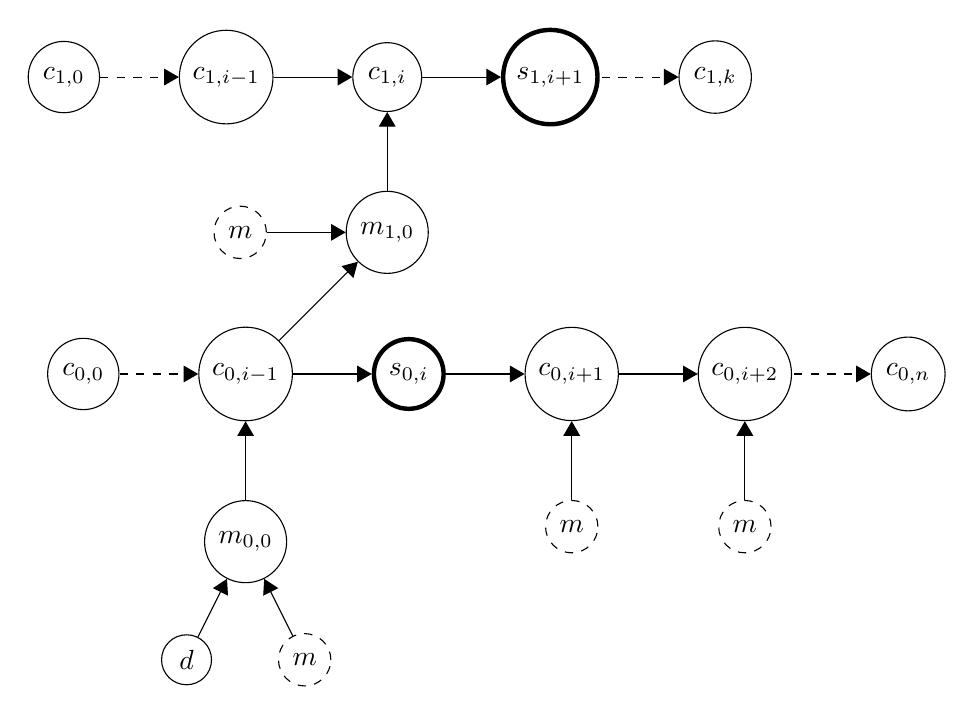
\begin{tikzpicture}[%level/.style={sibling distance=85mm/#1}, 
                                    every node/.style={circle,draw},
                                    every path/.style={<-,>=triangle 60}]

\node[ultra thick] (s0i) {$s_{0,i}$};

\node[left=of s0i] (c0iminus) {$c_{0,i-1}$} edge[->] (s0i);
\node[right=of s0i] (c0iplus) {$c_{0,i+1}$} edge[<-] (s0i);

\node[below=of c0iminus](c0m0) {$m_{0,0}$} edge[->] (c0iminus)
	child {node (d0) {$d$}}
	child {node[dashed] {$m$}};

\node[below=of c0iplus,dashed] {$m$} edge[->] (c0iplus);

\node[left=of c0iminus] (c0) {$c_{0,0}$} edge[->,dashed] (c0iminus);
\node[right=of c0iplus] (c0iplus2) {$c_{0,i+2}$} edge[<-] (c0iplus);

\node[below=of c0iplus2,dashed] {$m$} edge[->] (c0iplus2);

\node[right=of c0iplus2] (c0n) {$c_{0,n}$} edge[<-,dashed] (c0iplus2);


% second dag chain
\node[above right=of c0iminus] (c1m1) {$m_{1,0}$} edge[<-] (c0iminus);
\node[left=of c1m1,dashed] {$m$} edge[->] (c1m1);

\node[above=of c1m1] (c1i) {$c_{1,i}$} edge[<-](c1m1);
\node[left=of c1i] (c1iminus) {$c_{1,i-1}$} edge[->](c1i);
\node[left=of c1iminus] (c10) {$c_{1,0}$} edge[->,dashed](c1iminus);


\node[right=of c1i,ultra thick] (s1iplus) {$s_{1,i+1}$} edge[<-](c1i);

\node[right=of s1iplus] (c1k) {$c_{1,k}$} edge[<-,dashed](s1iplus);


\end{tikzpicture}